\chapter{Análisis}


\section{Metodología de desarrollo}

Las metodologías de desarrollo de software surgieron hace décadas como consecuencia de la acumulación de proyectos fallidos o de mala calidad, en los que los resultados no satisfacían al cliente. Esto era debido a que todo el desarrollo seguía el enfoque de los programadores del proyecto, los cuales no tenían en la mayoría de las ocasiones la misma visión que el cliente para el desarrollo del proyecto.

Hoy en día la elección de una metodología de desarrollo de software es fundamental para el desarrollo de un proyecto de calidad. El uso de una metodología, sin importar de que tipo sea, nos asegura que nuestro proyecto se adecuará a las peticiones del cliente y será un buen producto final.

La implantación de estas metodologías en la mayoría de los proyectos actuales ha aumentado el porcentaje de proyectos que terminan en éxito, y además en los plazos de tiempo establecidos.

\subsection{Tipos de metodologías}

Desde que empezó la preocupación por el desarrollo de los proyectos, distintas personas han investigado y desarrollado nuevas metodologías. Una posible clasificación de todas estas metodologías puede ser según la época de su creación, teniendo metodologías clásicas y metodologías ágiles.

\subsubsection{Metodología Clásica}

Las metodologías clásicas fueron las primeras metodologías que surgieron como solución al caos que había en la planificación de proyectos. La metodología clásica se caracteriza por una estructura secuencial, es decir, no se vuelve a la etapa anterior una vez se ha completado una etapa de la planificación; además el proceso es rígido y no cambia, es decir, una vez se acuerda como va a ser la planificación, a lo cual se le dedica grandes cantidades de tiempo, no se modifica nada de la planificación, ni siquiera los requisitos y, por lo tanto, la comunicación con el cliente se limita al comienzo del proyecto durante la elaboración de la planificación. Aunque, viendo su nombre, parezca que se trata de una metodología arcaica y en desuso, no es así bajo ningún concepto. Esta metodología se sigue puliendo y mejorando actualmente, aunque uno de sus problemas es su enfoque ''mayorista'', es decir, la metodología está enfocada a los macroproyectos. Un macroproyecto es un proyecto con una gran inversión, con un equipo de trabajo de varias decenas de personas, con los roles bien definidos; y con un amplio plazo de tiempo. Aunque un proyecto no encaje con la definición de macroproyecto, esta metodología se puede adaptar al proyecto en cuestión.

La metodología clásica o metodología ''en cascada'', recibiendo este nombre por la ausencia de vuelta a atrás en las etapas, su ciclo de etapas se puede visualizar en la Figura \ref{fig:etapas_clasica}.

\begin{figure}[h]
\centering
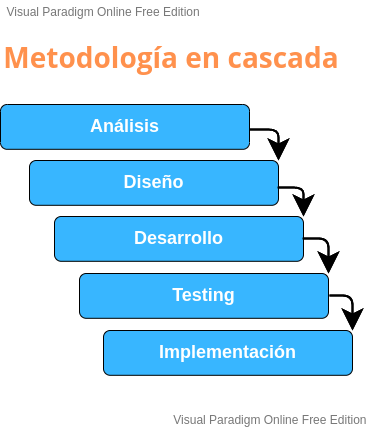
\includegraphics[width=0.7\textwidth]{imagenes/03_Analisis/meto_clasica.png}
\label{fig:etapas_clasica}
\begin{center}
Basado en: \url{https://www.yunbitsoftware.com/blog/2016/05/20/desarrolo-de-software-metodologias-waterfall-agile}
\end{center}
\caption{Etapas de la metodología clásica}
\end{figure}

Dado que la metodología clásica únicamente consta de un ciclo para realizar las etapas, será imprescindible una buena planificación de alcance, tiempo y coste del proyecto y de cada una de las etapas. Esta planificación inicial es tan importante porque no se obtendrán resultados del proyecto hasta que se encuentre cercano a su cierre.

Entre los problemas de la metodología clásica podemos encontrar los siguientes:

\begin{itemize}
\item Los proyectos de software reales difícilmente se adecuan a este modelo de proceso.
\item Dificultad para expresar por parte del cliente todos los requisitos al principio del proyecto.
\item Poca comunicación con cliente/usuario, hasta las etapas finales no hay un producto final que se pueda evaluar.
\end{itemize}

\subsubsection{Metodología Ágil}

Esta metodología surge como solución a los problemas de la metodología clásica, sobre todo para la planificación de proyectos cortos y cambiantes. La metodología ágil se caracteriza por su flexibilidad, durante el desarrollo del proyecto la planificación sufre continuos cambios debido a la constante comunicación con el cliente; una estructura incremental, con esta metodología no se obtiene un único proyecto final, si no más bien se van generando \glspl{prototipo} que se van analizando y mejorando en una retroalimentación constante, aumentando la colaboración; y un flujo de proceso iterativo, a diferencia de la metodología clásica donde cada etapa una vez finalizada no se vuelve a ella teniendo un flujo en cascada, en esta metodología el flujo de las etapas es más parecido a un círculo convertido en un bucle sin fin. Algo muy importante a tener en cuenta es que a pesar de que los sprints, un sprint es la realización de un ciclo completo; duren poco tiempo, esto no permite la ausencia de documentación, al igual que se hace en la metodología clásica, se debe documentar un mínimo a pesar de la brevedad de los sprints. Esta metodología se adapta mejor a los proyectos del ámbito de las \gls{TIC}, es decir, en el desarrollo de software, donde es fundamental la flexibilidad del proyecto y el carácter incremental de la metodología. Este modo de trabajar no se adecua a proyecto que puedan estar relacionados con sectores alejados de las \gls{TIC}, como puede ser el sector de la construcción, por ejemplo en la construcción de un puente, dado que no se pueden crear \glspl{prototipo} de una construcción, ya que no serían seguros, y además son proyectos poco cambiantes en los requisitos del proyecto durante su desarrollo.

El ciclo de etapas de la metodología ágil se puede visualizar en la Figura \ref{fig:etapas_agil}.

\begin{figure}[h]
\centering
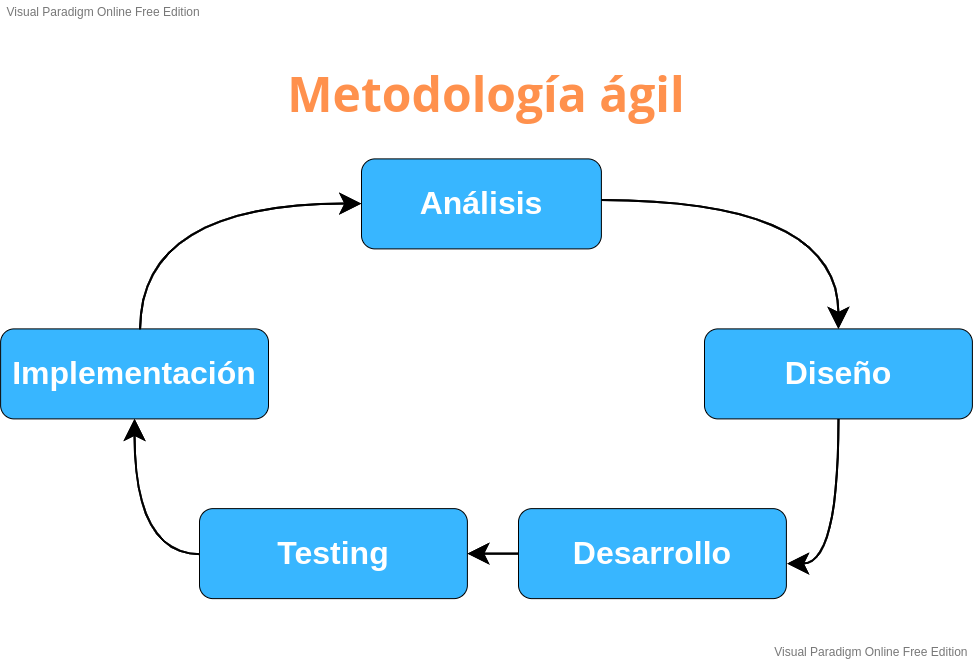
\includegraphics[width=0.9\textwidth]{imagenes/03_Analisis/meto_agil.png}
\label{fig:etapas_agil}
\begin{center}
Basado en: \url{https://www.yunbitsoftware.com/blog/2016/05/20/desarrolo-de-software-metodologias-waterfall-agile}
\end{center}
\caption{Etapas de la metodología ágil}
\end{figure}

Dentro de la categoría de metodología ágil podemos encontrar las siguientes metodologías:

\begin{itemize}
\item Scrum
\item Programación exterma (XP)
\item Mobile-D
\end{itemize}

En mi caso me voy a centrar en la metodología Scrum, muy popular hoy en día en la planificación de proyectos \gls{TIC}. Tal y como se indica en el artículo \cite{RefWorks:RefID:11-cevallos2018metodologias}, Scrum no corresponde a ningún acrónimo, su nombre proviene del rugby, es una formación requerida para la recuperación rápida del juego ante una infracción menor. Esta metodología se caracteriza por el empleo de un conjunto de reglas y la definición de roles. La existencia de estos roles favorece una colaboración eficaz del equipo de trabajo.
Los roles que se definen son: El Scrum master, el dueño del producto o Product owner y el equipo de desarrollo o team. El scrum master es la persona que lidera el equipo asegurándose que el equipo cumpla las reglas y procesos de la metodología. El dueño del producto es el representante de los accionistas y clientes que usan el software. El equipo de desarrollo es el grupo de profesionales encargados de convertir la lista de requerimientos o también llamado Product Backlog en funcionalidades del software \cite{RefWorks:RefID:11-cevallos2018metodologias}.

La característica incremental de las metodologías ágiles se materializa en la metodología Scrum como un elemento llamado Sprint (Figura \ref{fig:sprint_scrum}). Cada sprint consistirá en un recorrido completo de todas las etapas del proyecto, dando como resultado una versión funcional del producto.

Los elementos de un Sprint son los siguientes:

\begin{itemize}
\item Reunión de planificación del sprint
\item Daily Scrum o reunión diaria
\item Trabajo de desarrollo
\item Revisión
\item Retrospectiva del sprint
\end{itemize}

Durante la reunión de planificación del sprint se seleccionan que tareas se van a desarrollar en ese sprint. Las tareas son extraídas del Product Backlog, que no es más que una lista de tareas ordenas por prioridad. Esta lista será actualizada y modificada durante el desarrollo del proyecto.

\begin{figure}[h]
\centering
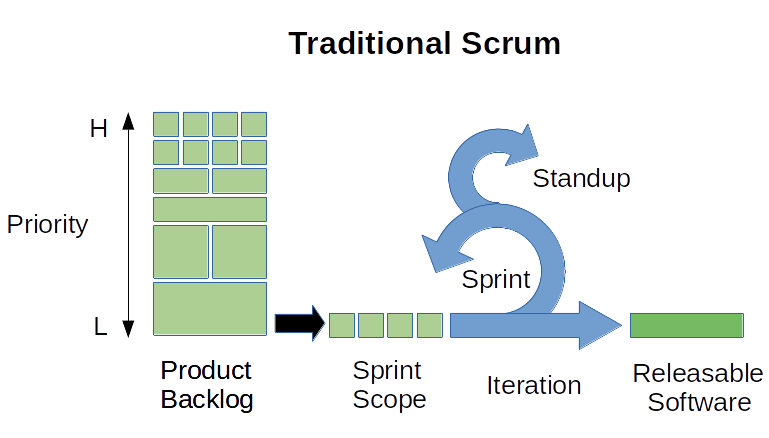
\includegraphics[width=1.0\textwidth]{imagenes/03_Analisis/sprint_scrum.png}
\begin{center}
Basado en: \url{https://openwebinars.net/blog/que-es-un-sprint-scrum}
\end{center}
\caption{Sprint de la metodología Scrum}
\label{fig:sprint_scrum}
\end{figure}


\subsection{Comparativa de las metodologías}

\begin{table}[h]
\centering
\resizebox{\textwidth}{!}{%
\begin{tabular}{|l|l|}
\hline
\rowcolor[HTML]{FFFC9E}
\multicolumn{1}{|c|}{\cellcolor[HTML]{FFFC9E}\textbf{Metodología Clásica}} &
\multicolumn{1}{c|}{\cellcolor[HTML]{FFFC9E}\textbf{Metodología Ágil}} \\ \hline
\begin{tabular}[c]{@{}l@{}}- Estructura secuencial o en cascada\\ - Proceso rígido\\ - Enfocada a macroproyectos\end{tabular} &
\begin{tabular}[c]{@{}l@{}}- Estructura incremental e iterativa\\ - Proceso flexible\\ - Enfocada a proyectos TIC\end{tabular} \\ \hline
\end{tabular}%
}
\caption{Comparativa de las metodologías de desarrollo}
\end{table}

\section{Aplicación de Scrum al proyecto} \label{sec:apli_scrum}

Tomando como partida la metodología Scrum original, se ha realizado una adaptación a mi proyecto. La primera adaptación es la asignación de roles, donde una misma persona efectúa los roles de Scrum master y el equipo de desarrollo, a la vez, este equipo de desarrollo lo formará una única persona; y por último, el papel de Product owner lo realizará el tutor del proyecto. Otra consecuencia, derivada de la formación del equipo por una única persona, es que no se van a hacer reuniones diarias, dado que no hay que proceder a una supervisión del trabajo del equipo en conjunto. Aunque no se hagan reuniones diarias, se ha optado por efectuar autorreflexiones semanalmente para llevar un control del avance durante el sprint. Los sprints tendrán una duración variable dependiendo de la cantidad y el peso de las tareas efectuadas en cada sprint. Además de las propias autorreflexiones, se harán reuniones con el tutor cada dos semanas, aunque el contacto con el tutor es constante durante todo el sprint vía correo electrónico.

\section{Historias de usuario} \label{sec:historias_usuario}

Dado que hemos elegido una metodología SCRUM las características y funcionalidades del sistema no van a estar definidas en función de una lista de requisitos, tal y como se hace en las metodologías tradicionales, indicando los requisitos funcionales, no funcionales y de información; sino que se van a definir por historias de usuario.

Las historias de usuario definen estos requisitos de una forma informal y desde el punto de vista de un rol. La historia de usuario estará formada por una serie de frases, pero la cantidad de frases será escasa, sin generalizar mucho en la funcionalidad descrita en la historia de usuario.

Las frases de las historias de usuario sigue el siguiente patrón: Como \textbf{<rol&gt;}, quiero \textbf{<evento&gt;} para \textbf{<funcionalidad&gt;}.

Además de la frase que describe la funcionalidad, una historia de usuario consta de una frase que indica cuando se considera completada la historia de usuario y de las tareas a realizar.

Una vez definida la estructura de las historias de usuario procedemos a describir cada una de ellas.


\subsection{Tarjetas de historias de usuario}

\begin{table}[H]
\centering
\resizebox{\textwidth}{!}{%
\begin{tabular}{|
>{\columncolor[HTML]{C0C0C0}}c |l|}
\hline
\textbf{Identificación} & HU.1 - Deducción de la edad                                                                                                         \\ \hline
\textbf{Descripción}    & \begin{tabular}[c]{@{}l@{}}Como usuario quiero que se deduzca mi edad \\ para personalizar las respuestas del chatbot.\end{tabular} \\ \hline
\textbf{Aceptación} &
  \begin{tabular}[c]{@{}l@{}}El sistema debe deducir la edad en \\ base a información proporcionada por el usuario \\ o en caso de no poder deducir esta información \\ deberá preguntar explícitamente al usuario.\end{tabular} \\ \hline
\textbf{Tareas} &
  \begin{tabular}[c]{@{}l@{}}• Añadir módulo de deducción al sistema antes \\    de comenzar la conversación temática.\\  • Comprobar que se ha deducido la información \\    antes de comenzar la conversación temática.\\  • Realizar la pregunta explícitamente si se \\     detecta que no se conoce la edad.\end{tabular} \\ \hline
\end{tabular}%
}
\caption{Historia de Usuario - HU.1}
\label{tab:HU1}
\end{table}

\begin{table}[H]
\centering
\resizebox{\textwidth}{!}{%
\begin{tabular}{|
>{\columncolor[HTML]{C0C0C0}}c |l|}
\hline
\textbf{Identificación} & HU.2 - Interfaz sencilla \\ \hline
\textbf{Descripción} & \begin{tabular}[c]{@{}l@{}}Como usuario quiero que la interfaz sea sencilla\\ para facilitar su uso por cualquier persona.\end{tabular} \\ \hline
\textbf{Aceptación}  & \begin{tabular}[c]{@{}l@{}}La interfaz debe tener una estructura de conversación\\ sencilla, de pregunta-respuesta.\end{tabular}        \\ \hline
\textbf{Tareas}      & \begin{tabular}[c]{@{}l@{}}• Integrar en el sistema una interfaz de conversación\\    estructuralmente sencilla.\end{tabular}           \\ \hline
\end{tabular}%
}
\caption{Historia de Usuario - HU.2}
\label{tab:HU2}
\end{table}

\begin{table}[H]
\centering
\resizebox{\textwidth}{!}{%
\begin{tabular}{|
>{\columncolor[HTML]{C0C0C0}}c |l|}
\hline
\textbf{Identificación} & HU.3 - Interfaz armónica                             \\ \hline
\textbf{Descripción} &
  \begin{tabular}[c]{@{}l@{}}Como usuario quiero que la interfaz siga la armonía\\ del sistema para que el uso de la misma sea \\ agradable para el usuario.\end{tabular} \\ \hline
\textbf{Aceptación} &
  \begin{tabular}[c]{@{}l@{}}La interfaz debe mantener la apariencia que tiene el\\ resto del sistema.\end{tabular} \\ \hline
\textbf{Tareas}         & • Integrar la apariencia del sistema en la interfaz. \\ \hline
\end{tabular}%
}
\caption{Historia de Usuario - HU.3}
\label{tab:HU3}
\end{table}

\begin{table}[H]
\centering
\resizebox{\textwidth}{!}{%
\begin{tabular}{|
>{\columncolor[HTML]{C0C0C0}}c |l|}
\hline
\textbf{Identificación} & HU.4 - Interfaz responsive          \\ \hline
\textbf{Descripción} &
  \begin{tabular}[c]{@{}l@{}}Como usuario quiero que la interfaz se adapte al\\ dispositivo que esté utilizando en cada momento\\ para aumentar el volumen de dispositivos con los\\ que podré utilizar el sistema.\end{tabular} \\ \hline
\textbf{Aceptación} &
  \begin{tabular}[c]{@{}l@{}}La interfaz debe adaptarse al tamaño de la pantalla\\ del dispositivo que esté utilizando el usuario.\end{tabular} \\ \hline
\textbf{Tareas}         & • Elaborar una interfaz responsive. \\ \hline
\end{tabular}%
}
\caption{Historia de Usuario - HU.4}
\label{tab:HU4}
\end{table}

\begin{table}[H]
\centering
\resizebox{\textwidth}{!}{%
\begin{tabular}{|
>{\columncolor[HTML]{C0C0C0}}c |l|}
\hline
\textbf{Identificación} &
  HU.5 - Conversación a tiempo real \\ \hline
\textbf{Descripción} &
  \begin{tabular}[c]{@{}l@{}}Como usuario quiero que la respuesta del sistema\\ se genere en un corto período de tiempo para\\ que su uso se haga más natural y entretenido.\end{tabular} \\ \hline
\textbf{Aceptación} &
  \begin{tabular}[c]{@{}l@{}}El sistema debe generar las respuestas y \\ proporcionárselas al usuario en un corto período de \\ tiempo que podría ser como máximo 5 segundos.\end{tabular} \\ \hline
\textbf{Tareas} &
  \begin{tabular}[c]{@{}l@{}}• Implementar un sistema eficiente en cuanto al\\ tiempo necesario para la generación de las res-\\ puestas.\end{tabular} \\ \hline
\end{tabular}%
}
\caption{Historia de Usuario - HU.5}
\label{tab:HU5}
\end{table}

\begin{table}[H]
\centering
\resizebox{\textwidth}{!}{%
\begin{tabular}{|
>{\columncolor[HTML]{C0C0C0}}c |l|}
\hline
\textbf{Identificación} &
  HU.6 - Conversación coherente \\ \hline
\textbf{Descripción} &
  \begin{tabular}[c]{@{}l@{}}Como usuario quiero que las respuestas del sistema\\ tenga una coherencia con el resto de la conversación \\ realizada con anterioridad a la pregunta para que su \\ uso sea más agradable e interesante para el usuario.\end{tabular} \\ \hline
\textbf{Aceptación} &
  \begin{tabular}[c]{@{}l@{}}Las respuestas del sistema deben tener cierta coherencia\\ con la conversación realizada hasta ese momento, \\ haciendo uso de la información proporcionada por el\\ usuario para generar la respuesta.\end{tabular} \\ \hline
\textbf{Tareas} &
  \begin{tabular}[c]{@{}l@{}}• Implementar un mecanismo que incluya la información\\ proporcionada por el usuario en la generación de las \\ respuestas.\\  • Implementar un mecanismo que genere distintas repues-\\ tas según la información deducida del usuario por el \\ módulo de deducción.\end{tabular} \\ \hline
\end{tabular}%
}
\caption{Historia de Usuario - HU.6}
\label{tab:HU6}
\end{table}

\begin{table}[H]
\centering
\resizebox{\textwidth}{!}{%
\begin{tabular}{|
>{\columncolor[HTML]{C0C0C0}}c |l|}
\hline
\textbf{Identificación} &
  HU.7 - Conversación temática \\ \hline
\textbf{Descripción} &
  \begin{tabular}[c]{@{}l@{}}Como administrador del sistema quiero que el sistema \\ genere respuestas relacionadas con la temática del \\ chatbot para favorecer el aprendizaje por parte del \\ usuario sobre la temática.\end{tabular} \\ \hline
\textbf{Aceptación} &
  \begin{tabular}[c]{@{}l@{}}El sistema debe orientar las respuestas hacia el ámbito \\ temático del chatbot, sin importar que pregunta se \\ haya realizado.\end{tabular} \\ \hline
\textbf{Tareas} &
  \begin{tabular}[c]{@{}l@{}}• Implementar un sistema que sea capaz de orientar las\\ respuestas a la temática del chatbot.\\  • Implementar un sistema que genere respuestas sobre\\ la temática del chatbot, personalizándolas al usuario en \\ base a la información proporcionada por el mismo.\end{tabular} \\ \hline
\end{tabular}%
}
\caption{Historia de Usuario - HU.7}
\label{tab:HU7}
\end{table}


\subsection{Listado de las historias de usuario}

Una vez se han definido todas las historias de usuario debemos clasificar las historias de usuario por algún criterio para decidir cuáles tienen un mayor impacto en el sistema y decidir cuáles abarcar en un primer momento a la hora de ser implementadas las funcionalidades descritas en las historias. Este criterio será el nivel de prioridad. El nivel de prioridad toma valores desde 1 hasta 3, donde 1 es el mínimo nivel de prioridad y 3 el máximo nivel de prioridad. Este listado se puede ver en la Tabla \ref{tab:listado_HU}.

\begin{table}[h]
\centering
\resizebox{\textwidth}{!}{%
\begin{tabular}{|c|l|c|}
\hline
\rowcolor[HTML]{C0C0C0}
\textbf{Identificador} &
\multicolumn{1}{c|}{\cellcolor[HTML]{C0C0C0}\textbf{Descripción}} &
\textbf{Prioridad} \\ \hline
HU.1 (Tabla \ref{tab:HU1}) &
\begin{tabular}[c]{@{}l@{}}Como usuario quiero que se deduzca mi edad\\ para personalizar las respuestas del chatbot.\end{tabular} &
3 \\ \hline
HU.2 (Tabla \ref{tab:HU2}) &
\begin{tabular}[c]{@{}l@{}}Como usuario quiero que la interfaz sea sencilla\\ para facilitar su uso por cualquier persona.\end{tabular} &
2 \\ \hline
HU.3 (Tabla \ref{tab:HU3}) &
\begin{tabular}[c]{@{}l@{}}Como usuario quiero que la interfaz siga la armonía\\ del sistema para el uso de la misma sea agradable\\ para el usuario.\end{tabular} &
1 \\ \hline
HU.4 (Tabla \ref{tab:HU4}) &
\begin{tabular}[c]{@{}l@{}}Como usuario quiero que la interfaz se adapte al\\ dispositivo que esté utilizando en cada momento\\ para aumentar el volumen de dispositivos con los \\ que podré utilizar el sistema.\end{tabular} &
2 \\ \hline
HU.5 (Tabla \ref{tab:HU5}) &
\begin{tabular}[c]{@{}l@{}}Como usuario quiero que la respuesta del sistema\\ se genere en un corto período de tiempo para\\ que su uso se haga más natural y entretenido.\end{tabular} &
3 \\ \hline
HU.6 (Tabla \ref{tab:HU6}) &
\begin{tabular}[c]{@{}l@{}}Como usuario quiero que las respuestas del sistema\\ tenga una coherencia con el resto de la conversación\\ realizada con anterioridad a la pregunta para que su \\ uso sea más agradable e interesante para el usuario.\end{tabular} &
3 \\ \hline
HU.7 (Tabla \ref{tab:HU7}) &
\begin{tabular}[c]{@{}l@{}}Como administrador del sistema quiero que el sistema\\ genere respuestas relacionadas con la temática del chatbot\\ para favorecer el aprendizaje por parte del usuario sobre \\ la temática.\end{tabular} &
2 \\ \hline
\end{tabular}%
}
\caption{Listado de historias de usuario junto con su prioridad}
\label{tab:listado_HU}
\end{table}

\section{Requisitos adicionales}

\begin{itemize}
\item \textbf{Robustez:} El chatbot deberá responder siempre sin importar que mensaje envíe el usuario.
\item \textbf{Documentación:} Se incluirá información a modo de manual de usuario para facilitar la utilización del sistema y el ajuste de sus parámetros.
\item \textbf{Extensibilidad:} El chatbot debe estar preparado para ser fácilmente escalado y tener la suficiente potencia para cumplir sus requisitos.
\item \textbf{Costo:} El costo final de implementación del sistema debe ser bajo, para ello el sistema debe usar la menor cantidad de recursos de pago sin perder la potencia necesaria.
\item \textbf{Seguridad:} Se deben mantener privados todos los datos proporcionados por el usuario durante el uso del sistema.
\end{itemize}

\section{Análisis de riesgos}

Una problemática de la que ningún proyecto se puede escapar es la aparición de continuos riesgos durante el desarrollo del mismo, que pueden ocasionar problemas en el desarrollo del proyecto. Pero esto no quiere decir que estos riesgos se tenga que materializar siempre. Por esta razón existe el análisis de riesgos, para detectarlos y poner medidas para minimizar la probabilidad de su aparición.

Este análisis de riesgos consiste en detectar los riesgos que puedan apareces, analizar las posibles causas que pueden originar este riesgo, y por último, elaborar un plan de actuación para evitar la aparición del riesgo asociado a ese plan de actuación.

Tras realizar el análisis de riesgos se obtendrá una lista de riesgos, esta lista de riesgos se materializa como una tabla (Tabla \ref{tab:tabla_riesgos}) que sigue el esquema Riesgo-Causa-Actuación. Además, se clasifican los distintos riesgos en una matriz de probabilidad-impacto (Tabla \ref{tab:matriz_probabilidad_impacto}).

\begin{table}[h]
\centering
\resizebox{\textwidth}{!}{%
\begin{tabular}{|c|l|l|l|}
\hline
\rowcolor[HTML]{C0C0C0} 
\textbf{Identificador} &
  \multicolumn{1}{c|}{\cellcolor[HTML]{C0C0C0}\textbf{Riesgo}} &
  \multicolumn{1}{c|}{\cellcolor[HTML]{C0C0C0}\textbf{Causa}} &
  \multicolumn{1}{c|}{\cellcolor[HTML]{C0C0C0}\textbf{Plan de actuación}} \\ \hline
R.1 &
  \begin{tabular}[c]{@{}l@{}}Falta de información para generar el conjunto de datos con el \\ que entrenar el chatbot\end{tabular} &
  \begin{tabular}[c]{@{}l@{}}Uso del chatbot en temas muy especializados y \\ poco discutidos en Internet\end{tabular} &
  \begin{tabular}[c]{@{}l@{}}Intentar usar el chatbot con temas frecuentes \\ en foros de Internet\end{tabular} \\ \hline
R.2 &
  Pérdida del proyecto &
  \begin{tabular}[c]{@{}l@{}}Fallos en los equipos que contienen la \\ información del proyecto o pérdidas de los mismos\end{tabular} &
  \begin{tabular}[c]{@{}l@{}}Utilizar herramientas de \gls{backup} para tener \\ siempre una copia de seguridad\end{tabular} \\ \hline
R.3 &
  \begin{tabular}[c]{@{}l@{}}Pérdida del listado de cambios realizados en el \\ proyecto\end{tabular} &
  Realizar el proyecto sin guardar versiones del mismo &
  \begin{tabular}[c]{@{}l@{}}Utilizar herramientas de control de versiones \\ como Github\end{tabular} \\ \hline
R.4 &
  Complejidad tecnológica &
  \begin{tabular}[c]{@{}l@{}}Desconocimiento de la tecnología base del \\ proyecto o inmadurez de la tecnología utilizada\end{tabular} &
  \begin{tabular}[c]{@{}l@{}}Realizar un análisis previo de las tecnologías \\ a utilizar en el proyecto para analizar su \\ viabilidad de uso en el proyecto\end{tabular} \\ \hline
R.5 &
  \begin{tabular}[c]{@{}l@{}}Solicitud de cambios continuos por parte del \\ cliente\end{tabular} &
  \begin{tabular}[c]{@{}l@{}}Mala comunicación con el cliente o falta de \\ entendimiento entre ambas partes\end{tabular} &
  \begin{tabular}[c]{@{}l@{}}Realizar reuniones frecuentas para el análisis \\ del estado del proyecto y mantener un flujo de \\ \gls{feedback} continuo con el cliente\end{tabular} \\ \hline
R.6 &
  \begin{tabular}[c]{@{}l@{}}Falta de conocimientos por parte del cliente sobre la \\ tecnología en que se basa el proyecto\end{tabular} &
  \begin{tabular}[c]{@{}l@{}}Uso de tecnologías muy técnicas y \\ especializadas, o de reciente aparición\end{tabular} &
  \begin{tabular}[c]{@{}l@{}}Analizar los conocimientos del cliente al inicio \\ del proyecto y tratar de explicar de una forma \\ sencilla las bases de las tecnologías utilizadas\end{tabular} \\ \hline
R.7 &
  Los objetivos del proyecto no son realistas &
  Sobreestimación del alcance del proyecto &
  \begin{tabular}[c]{@{}l@{}}Realizar una planificación coherente con el \\ tiempo y recursos disponibles\end{tabular} \\ \hline
R.8 &
  Generación de las respuestas en un tiempo excesivo &
  Utilización de tecnologías lentas y poco eficientes &
  \begin{tabular}[c]{@{}l@{}}Realizar optimizaciones en la generación de \\ respuestas\end{tabular} \\ \hline
R.9 &
  \begin{tabular}[c]{@{}l@{}}Problemas puntuales con las herramientas de \\ comunicación\end{tabular} &
  Caídas del servicio de correo o de videollamada &
  \begin{tabular}[c]{@{}l@{}}Buscar herramientas alternativas a las \\ herramientas que están teniendo problemas \\ puntuales\end{tabular} \\ \hline
R.10 &
  Quejas sobre la interfaz del sistema &
  Implementación poco intuitiva de la interfaz &
  \begin{tabular}[c]{@{}l@{}}Evaluación de los prototipos de interfaz por \\ parte del cliente\end{tabular} \\ \hline
R.11 &
  Fugas de información sobre los usuarios &
  \begin{tabular}[c]{@{}l@{}}Mala gestión en la seguridad de los datos \\ gestionados por el sistema\end{tabular} &
  \begin{tabular}[c]{@{}l@{}}Intentar conservar la mínima cantidad de \\ información en el sistema, y aquella información \\ que se necesite conservar guardarla con la mayor \\ seguridad posible\end{tabular} \\ \hline
R.12 &
  Aparición de tareas imprevistas &
  \begin{tabular}[c]{@{}l@{}}Planificación errónea basada en un mal análisis del\\ proyecto\end{tabular} &
  \begin{tabular}[c]{@{}l@{}}Replanificar las tareas y actualizar tanto el\\ backlog como los sprints a realizar\end{tabular} \\ \hline
R.13 &
  \begin{tabular}[c]{@{}l@{}}Los modelos no llegan a cumplir con las \\ expectativas\end{tabular} &
  \begin{tabular}[c]{@{}l@{}}Dificultad para entrenar los modelos en la tarea que\\ se tiene pensada en un principio\end{tabular} &
  \begin{tabular}[c]{@{}l@{}}Dedicar un mayor tiempo a la búsqueda de \\ información y a la labor de entrenamiento de los\\ modelos\end{tabular} \\ \hline
R.14 &
  \begin{tabular}[c]{@{}l@{}}Finalización de los periodos de prueba gratuitos de\\ ciertas herramientas\end{tabular} &
  \begin{tabular}[c]{@{}l@{}}Extensión del periodo de tiempo de uso de las\\ herramientas\end{tabular} &
  \begin{tabular}[c]{@{}l@{}}Realizar una buena planificación del inicio de los\\ periodos de prueba acorde al ritmo de trabajo del\\ proyecto\end{tabular} \\ \hline
R.15 &
  Deducción errónea de la edad del usuario &
  \begin{tabular}[c]{@{}l@{}}Mala calidad de la imagen tomada por el usuario o\\ uso de un modelo poco preciso para la clasificación\\ de personas mediante la edad\end{tabular} &
  \begin{tabular}[c]{@{}l@{}}Mostrar al usuario la imagen que va a enviar al\\ proceso de deducción, y buscar modelos probados\\ que tengan una fiabilidad y precisión aceptables\end{tabular} \\ \hline
\end{tabular}%
}
\caption{Tabla de riesgos del proyecto}
\label{tab:tabla_riesgos}
\end{table}

\begin{table}[h]
\centering
\resizebox{\textwidth}{!}{%
\begin{tabular}{|
>{\columncolor[HTML]{C0C0C0}}c |
>{\columncolor[HTML]{32CB00}}c |c|c|c|c|}
\hline
\textbf{\begin{tabular}[c]{@{}c@{}}Probabilidad \rightarrow\\ Impacto \downarrow\end{tabular}} &
  \cellcolor[HTML]{C0C0C0}\textbf{0,1} &
  \cellcolor[HTML]{C0C0C0}\textbf{0,3} &
  \cellcolor[HTML]{C0C0C0}\textbf{0,5} &
  \cellcolor[HTML]{C0C0C0}\textbf{0,7} &
  \cellcolor[HTML]{C0C0C0}\textbf{0,9} \\ \hline
\textbf{Muy Bajo} &     & \cellcolor[HTML]{32CB00}R.9 & \cellcolor[HTML]{32CB00}     & \cellcolor[HTML]{FCFF2F} & \cellcolor[HTML]{FCFF2F} \\ \hline
\textbf{Bajo}     &     & \cellcolor[HTML]{32CB00}R.6 & \cellcolor[HTML]{FCFF2F}     & \cellcolor[HTML]{FCFF2F} & \cellcolor[HTML]{F8A102} \\ \hline
\textbf{Medio}    & R.5 & \cellcolor[HTML]{FCFF2F}R.3 & \cellcolor[HTML]{FCFF2F}R.10 & \cellcolor[HTML]{F8A102} & \cellcolor[HTML]{F8A102} \\ \hline
\textbf{Alto} &
  \cellcolor[HTML]{FCFF2F}R.12 &
  \cellcolor[HTML]{FCFF2F}\begin{tabular}[c]{@{}c@{}}R.4\\ R.14\\ R.15\end{tabular} &
  \cellcolor[HTML]{F8A102}R.7 &
  \cellcolor[HTML]{F8A102}\begin{tabular}[c]{@{}c@{}}R.1\\ R.13\end{tabular} &
  \cellcolor[HTML]{FE0000} \\ \hline
\textbf{Muy Alto} &
  \cellcolor[HTML]{FCFF2F}R.2 &
  \cellcolor[HTML]{F8A102} &
  \cellcolor[HTML]{F8A102}\begin{tabular}[c]{@{}c@{}}R.8 \\ R.11\end{tabular} &
  \cellcolor[HTML]{FE0000} &
  \cellcolor[HTML]{FE0000} \\ \hline
\end{tabular}%
}
\caption{Matriz probabilidad-impacto de riesgos}
\label{tab:matriz_probabilidad_impacto}
\end{table}



\section{Riesgos materializados}

Durante el trascurso del proyecto no se han materializado riesgos en gran cantidad, aunque en la etapa final si se han materializado algunos de ellos. Los riesgos materializados se han centrado sobre todo en los modelos que generan las respuestas desde distintos puntos. Uno de los primeros riesgos que se manifestó fue el riesgo de generar las respuestas en un tiempo excesivo (R.8). A pesar de su materialización, aplicando el plan de actuación previsto se pudo solucionar rápidamente. Este plan de actuación consiste en emplear módulos de optimización para mejorar los tiempos de inferencia de estos módulos, en concreto, el módulo de optimización utilizado es DeepSpeed, del cual se hablará en posteriores apartados del proyecto.

Finalmente, se materializaron dos riesgos muy relacionados entre ellos. El riesgo que en principio origina al otro riesgo, es el riesgo de la falta de información para generar los conjuntos de datos necesarios para entrenar a los modelos (R.1). Sí que se han llegado a generar conjuntos de datos, pero dada la dificultad y el alto gasto de tiempo necesario no se ha llegado a cumplir el objetivo del todo y, por lo tanto, se ha materializado en parte este riesgo. Esta materialización provoca la materialización del riesgo de no cumplir con las expectativas puestas en los modelos del chatbot. Puesto que no se llega a conseguir el conjunto de datos buscado, no se podrá tener el modelo buscado. Como adelanto a lo que se tratará en posteriores apartados, se buscaba que los modelos fuesen capaces de enfocar la conversación a un tono didáctico basándose en la información que le iba proporcionando el usuario durante la conversación, pero finalmente no se ha conseguido obtener esos modelo con un cierto enfoque didáctico. También el riesgo de no cumplir las expectativas que se tuvieran sobre los modelos conversacionales del chatbot llevan implícito el riesgo de haber impuesto unos objetivos poco realistas (R.7). Sin duda, puede que se hayan fijado objetivos difícilmente alcanzables en el tiempo disponible para el desarrollo de este proyecto, puesto que implementar un chatbot que sea capaz de realizar una función con cierto grado de complejidad no es una tarea sencilla y rápida, sobre todo no es rápida porque hay que hacer gran hincapié en lo costoso que es obtener información de calidad y que se encuentre en grandes cantidades.


